% !TEX encoding = UTF-8
% !TEX TS-program = pdflatex
% !TEX root = ../arsclassica.tex
% !TEX spellcheck = it-IT

%************************************************
\chapter{Creazione di dataset relativi al traffico}
\label{cap:tsis-sensors}
%************************************************
Al fine di valutare le prestazioni degli algoritmi di apprendimento e classificazione delle \acl{CTBN} è emersa la necessità di generare dei dataset adeguati a tale scopo.

Come già specificato in precedenza, le \acs{CTBN} sono un modello stocastico dedito alla rappresentazione dell'evoluzione di sistemi dinamici, cioè di fenomeni cangianti nel tempo (non necessariamente o esclusivamente in base ad esso) rappresentabili come insiemi di traiettorie multi-variate. Si è quindi scelto di generare dei dataset che rappresentassero un tipico sistema cangiante: il traffico automobilistico su rete stradale.

Tali dataset, costituiti da un insieme di documenti rappresentanti la presenza (durante l'evolvere del tempo) di veicoli sui sensori di una rete stradale, sono stati generati con l'ausilio di un software commerciale, \acf{TSIS} (versione $\geq$ 6.2) e di una sua \acl{RTE} appositamente sviluppata al fine di monitorare e tracciare il passaggio dei veicoli. 

In questo capitolo si presentano sia i succitati strumenti utilizzati per la creazione di reti stradali e relativi modelli di simulazione, sia lo strumento creato per la creazione di dataset relativi al traffico.

Relativamente, invece, al processo pratico di creazione dei dataset si rimanda alla~\autoref{sec:create-dataset-howto}.

\section{TSIS}
\label{sec:tsis}
\acf{TSIS} è un \acl{IDE}\footnote{Un \acl{IDE}, comunemente chiamato anche \ACF{IDE}, è un insieme di programmi finalizzati a supportare il processo di sviluppo dei software. Generalmente, un \acs{IDE} è costituito da uno strumento per la creazione e modifica del codice sorgente, un compilatore o un interprete, strumenti per l'automazione dello sviluppo e la qualità del codice sorgente.}, distribuito commercialmente da McTrans\footnote{McTrans Moving Technology: \url{http://mctrans.ce.ufl.edu}.} e supportato dalla \acf{FWHA}\footnote{Agenzia del Dipartimento dei Trasporti degli Stati Uniti d'America: \\ \url{www.fhwa.dot.gov}.}, il cui scopo ultimo è permettere la simulazione e l'analisi di modelli di reti stradali.

\acs{TSIS} è costituito da insieme di strumenti dedicati alla creazione di reti stradali e relativi modelli di simulazione, all'esecuzione, e eventualmente alla visualizzazione, di tali modelli, così come all'interpretazione dei risultati ottenuti. Tale insieme di strumenti è reso accessibile tramite delle interfaccie grafiche\footnote{Un'interfaccia grafica, nota anche come \acf{GUI}, è un tipo di interfaccia utente il cui fine è permettere all'utente di interagire con il software manipolando oggetti grafici convenzionali.}.

L'architettura modulare con cui \acs{TSIS} è realizzato permette, in caso di necessità, di estendere tale ambiente creando degli ulteriori strumenti.

Di seguito si introducono brevemente i concetti relativi a \acs{TSIS} utilizzati nel prosieguo di questo lavoro di tesi.

Tuttavia si osservi che, poiché lo scopo di questa sezione non consiste nel documentare \acs{TSIS}, la sua trattazione esaustiva (\eg{}, semantica e lista completa dei tipi di dati rappresentabili) è omessa. A tale fine si rimanda invece alla documentazione ufficiale del software in questione.

\begin{definizione}[Progetto \acs{TSIS}]\label{defn:tsis-proj}
Un progetto \acs{TSIS} è un insieme di modelli di simulazione per una specifica rete stradale.
\end{definizione}

\begin{definizione}[Modello di simulazione \acs{TSIS}]\label{defn:tsis-sim-model}
Un modello di simulazione è costituito da un input (\eg{}, variazioni dei flussi di ingresso nella rete, variazioni delle percentuali di svolta dei veicoli nelle intersezioni) per la simulazione di una determinata rete stradale e tutti i dati generati dalla sua esecuzione (\ie{}, simulazione).
\end{definizione}
\begin{osservazione}
Un modello di simulazione può anche prevedere che la sua esecuzione sia eseguita più volte. Finché il seme dei numeri casuali non è modificato, esso è sempre considerato un singolo modello di simulazione.
\end{osservazione}

\begin{definizione}[Formato \acs{TRF}]\label{defn:trf-format}
\acs{TRF}\footnote{\acf{TRF}.} è il formato dei file accettati dal simulatore di \acs{TSIS}. Esso codifica e rappresenta una rete stradale e il relativo modello di simulazione specificandone i vari componenti tramite l'utilizzo dei rispettivi \acs{RT} (si veda la~\vref{defn:tsis-rt}).
\end{definizione}
\begin{osservazione}
Il formato \acs{TRF} è equivalente al formato \acs{TRAF}\footnote{\acf{TRAF}.}.
\end{osservazione}

\begin{definizione}[Formato \acs{TNO}]\label{defn:tno-format}
\acs{TNO}\footnote{\acf{TNO}.} è il formato nativo con cui vengono rappresentate in memoria le reti stradali create visivamente tramite l'interfaccia grafica \acs{TRAFED}.
\end{definizione}

\begin{definizione}[\acl{RT}]\label{defn:tsis-rt}
Un \acf{RT} rappresenta il blocco informativo minimo su cui è costruita una rete stradale e il suo modello di simulazione. Nel concreto esso consiste in una singola riga di testo nei file \acs{TRF} contenente un codice identificativo numerico e dei valori per i rispettivi campi accettati nell'ordine prestabilito. Allo stesso modo, tale formato descrive anche il modello di simulazione della rete stradale.
\end{definizione}

\subsection{Componenti}
In questa sezione si elencano gli strumenti che costituiscono l'ambiente di sviluppo \acs{TSIS}.

\begin{description}
\item[CORSIM] \hfill \\
\acs{CORSIM}\footnote{\acf{CORSIM}.} costituisce il componente principale dell'insieme di strumenti denominato \acs{TSIS}. È un simulatore il cui obiettivo è permettere la creazione e l'esecuzione di modelli di simulazione \acs{TSIS}. È composto da due simulatori integrati che rappresentano l'intero sistema di traffico come funzione del tempo: \acs{NETSIM}\footnote{\acf{NETSIM}.} e \acs{FREESIM}\footnote{\acf{FREESIM}.}. Tali simulatori integrati rappresentano, rispettivamente, il traffico sulle strade urbane e non. La simulazione effettuata da tali strumenti è di tipo microscopico: essi modellano individualmente il comportamento di ogni singolo veicolo, prendendo in considerazione per ognuno di essi una serie di variabili, anche di tipo stocastico (\eg{}, tipologia di guidatore). Per tale motivo \acs{CORSIM} è dotato di molte possibili opzioni di configurazione e permette lo studio di modelli molto complessi e dettagliati.
\item[TRAFED] \hfill \\
\acs{TRAFED}\footnote{\acf{TRAFED}.} è una \acs{GUI} il cui scopo è permettere la creazione e la modifica di reti stradali e di modelli di simulazione per \acs{CORSIM}.
\item[TShell] \hfill \\
\acs{TShell}\footnote{\acf{TShell}.} è la \acs{GUI} di \acs{TSIS}. Funge da contenitore degli strumenti (preconfigurati, o creati dall'utente) di questo ambiente di sviluppo integrato e permette la gestione dei progetti \acs{TSIS}.
\item[TRAFVU] \hfill \\
\acs{TRAFVU}\footnote{\acf{TRAFVU}.} è una \acs{GUI} finalizzata alla visualizzazione dei modelli di simulazione simulati con \acs{CORSIM}. Essa permette sia di visualizzare in modo animato l'evoluzione del traffico nella rete stradale con una qualsiasi granularità temporale, sia di visualizzare una serie di misure di interesse relative alla simulazione.
\item[TSIS Text Editor] \hfill \\
\acs{TSIS} \acsfont{Text Editor} è uno strumento il cui scopo è facilitare la modifica manuale dei file \acs{TRF}. A tale scopo esso visualizza per ogni \acs{RT} che si intende modificare sia la sua descrizione sia l'insieme dei campi supportati.
\item[TSIS Script Tool] \hfill \\
\acs{TSIS} \acsfont{Script Tool} è uno strumento per la creazione, la modifica e l'esecuzione di codice \acs{VBScript}\footnote{\acf{VBScript} è un linguaggio interpretato, sottoinsieme del linguaggio \emph{Visual Basic}, utilizzato come sostituto o integrazione della linea di comando o per il controllo di applicazioni esterne in ambiente \emph{Microsoft Windows}.}. Questo strumento fornisce un meccanismo utile ad automatizzare le funzionalità di simulazione di \acs{TSIS} (\eg{}, esecuzioni multiple dello stesso modello di simulazione variando il seme dei numeri casuali che governa la distribuzione di ingresso dei veicoli nella rete stradale).
\item[TSIS Translator] \hfill \\
\acs{TSIS} \acsfont{Translator} è uno strumento utile alla conversione dei file dal formato \acs{TRF} al formato \acs{TNO} e viceversa. Tale operazione risulta utile al fine di rendere i file \acs{TRF} utilizzabili tramite lo strumento \acs{TRAFED} così come per rendere i file \acs{TNO} utilizzabili con \acs{CORSIM}.
\item[TSIS Output Processor] \hfill \\
\acs{TSIS} \acsfont{Output Processor} è uno strumento finalizzato alla raccolta e l'aggregazione dei dati da \acs{CORSIM} durante l'esecuzione multipla di modelli di simulazione. La sua caratteristica principale consiste nella computazione automatica di un insieme di statistiche predefinite. Esso permette di scegliere sia le statistiche di interesse sia la granularità temporale della loro computazione.
\end{description}

\subsection{Caratteristiche}
Segue una panoramica il cui scopo è presentare sia le principali capacità, sia i vincoli di modellazione, simulazione e analisi di \acs{TSIS}.

\acs{TSIS}, tramite \acs{CORSIM}, permette la modellazione di reti stradali con le seguenti caratteristiche:

\begin{itemize}
	\item reti stradali urbane, non urbane o miste
	\item controllo quantitativo (\ie{}, quantità di veicoli per intervallo temporale, distribuita secondo una distribuzione statistica) e qualitativo (\ie{}, tipo di veicoli) dei flussi di veicoli in ingresso nella rete stradale
	\item controllo completo del flusso di traffico (\ie{}, percentuali di svolta dei veicoli variabile nel tempo)
	\item supporto per strade con più corsie (massimo $9$)
	\item supporto dei segnali stradali
	\item supporto per gli attraversamenti pedonali
	\item intersezioni non controllate
	\item intersezioni controllate da semafori
	\item canalizzazione delle corsie
	\item piani semaforici predefiniti, dinamici (\eg{}, priorità ai veicoli di emergenza) o guidati da algoritmi (\eg{}, attivazione del semaforo in base alle rilevazioni effettuate dai sensori)
	\item sensori per la rilevazione del passaggio o della presenza di veicoli
	\item supporto per i mezzi di trasporto pubblico (\ie{}, autobus, taxi)
	\item rilevamento di incidenti
	\item supporto per i sistemi di guida anglosassoni
	\item simulazione guidata all'analisi delle code
	\item simulazione guidata allo studio del grado di occupazione della rete stradale
	\item output di dati di interesse aggregati
	\item output di dati statistici collezionati
\end{itemize}

Poiché un modello di simulazione del traffico è caratterizzato dal cambiamento di un insieme di condizioni (\eg{}, volumi di traffico, canalizzazione delle corsie, percentuali di svolta dei veicoli) della rete stradale, esso deve specificare, oltre alla natura stessa dei cambiamenti, anche i fattori in base a cui essi avvengono. Il fattore principale che viene preso in considerazione è il tempo. Ne consegue perciò che un modello di simulazione del traffico deve specificare l'intervallo temporale in cui specifici cambiamenti di determinate condizioni avvengono.

\acs{CORSIM} affronta questo problema permettendo di partizionare il tempo totale di simulazione in una serie di periodi temporali (\ie{}, \emph{time period}) di durata variabile. Ogni periodo temporale possiede perciò un insieme di dati di input che non variano per tutta la sua durata. Inoltre, i periodi temporali sono a loro volta suddivisi in intervalli temporali (\ie{}, \emph{time interval}), anch'essi suddivisi in passi temporali (\ie{}, \emph{time step}). 

La granularità massima con cui \acs{CORSIM} e \acs{TSIS} \acsfont{Output Processor} sono in grado di raccogliere dati e computare statistiche cumulative è collegata ...

Tuttavia, le principali limitazioni di \acs{TSIS} derivano esattamente dalle modalità con cui \acs{CORSIM} implementa la gestione del tempo: la lista dei periodi temporali è rappresentata internamente tramite un array statico di dimensione prefissata. Nello specifico, un modello \acs{CORSIM} può essere costituito da un massimo di $19$ periodi temporali, ognuno dei quali con una durata compresa tra i $10$ e i $9999$ secondi: ciò implica che non è possibile eseguire modelli di simulazione che si protraggono oltre un tempo di circa $52$ ore.

%Each time period is subdivided into a sequence of time intervals. The output of cumulative simulation statistics is
%only available on a time interval basis (see Record Type 05). The time interval duration is typically set to the most
%common signal cycle length in a study network. The duration of each time period must be at least one time interval,
%as specified on Record Type 04. Furthermore, the duration of each time period must be an integer multiple of the
%time interval duration. The program will automatically guarantee this requirement by truncating each time period
%%duration to the nearest integer multiple of the time interval duration. (See the following figure for the relationship
%between the time period, the time interval, and the time step.)

%RT 04, campo 1
%This entry specifies the number of FRESIM time steps per second.
%NETSIM was designed to operate at a fixed 1-second time step, while FRESIM was designed to operate at a user-
%specified time step duration in the range 0.1 to 1.0 seconds. However, to keep both NETSIM and FRESIM
%synchronized, the duration of the FRESIM time step cannot be arbitrarily set to any value in the range [0.1, 1.0].
%Rather than specifying the duration of the FRESIM time step, this entry is used to specify the number of FRESIM
%time steps that are executed for every second of simulation time. Using this approach, smaller duration time steps
%can be applied to FRESIM while keeping both NETSIM and FRESIM properly synchronized. The following table
%provides the equivalent FRESIM time step duration for each valid value for this entry.

\begin{figure}
\centering
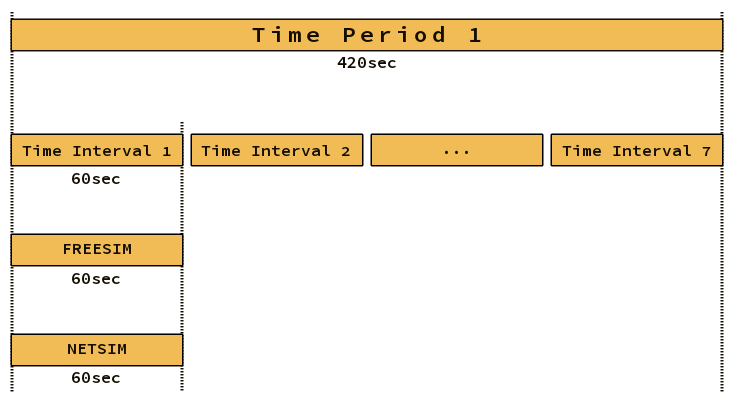
\includegraphics[width=1\columnwidth]{corsim-time}
\caption[Gestione del tempo in \acs{CORSIM}]{Esempio di suddivisione gerarchica delle unità temporali in \acs{CORSIM}. Un \emph{time period} della durata di $420$ secondi è suddiviso in $7$ \emph{time interval}, ciascuno della durata di $60$ secondi.}
\label{fig:corsim-time}
\end{figure}

%inserire riferimenti alla documentazione, # RT

\subsection{Estendere TSIS}
% panoramica sviluppo RTE
% TODO: descrizione delle varie API fornite da TSIS
% in questa sezione presentaimo il funzionamento dell'interfacciamento tra CORSIM e strumenti esterni (CORSIM RTE) più dettagliatamente perché ci interessano al fine di ...
% presentiamo le API fornite dall'ambiente di sviluppo di TSIS
% mettere immagine di pulsante sensors in TSIS? far vedere come si aggiunge una RTE all'ambiente di TSIS (piccola sezione)

Come accennato, \acs{TSIS} espone un meccanismo finalizzato all'estensione delle sue funzionalità tramite la creazione, da parte dell'utente, di altri strumenti da integrare nell'ambiente di sviluppo. Tali strumenti, interfacciandosi direttamente con \acs{CORSIM}, possono modificarne o aumentarne la logica di simulazione, collezionare dati o monitorare eventi speciali (\eg{}, indicenti).

In questa sottosezione si presenta dapprima il funzionamento dei meccanismi di interfacciamento tra \acs{CORSIM} e strumenti esterni, a cui ci si riferirà da questo momento in poi con il termine \acs{CORSIM} \acs{RTE}\footnote{\ACF{RTE}.}. La discussione, in seguito, verterà sulle modalità di creazione delle \acs{CORSIM} \acs{RTE} sviluppata per la creazione dei dataset.

La~\vref{fig:tsis-corsim-arch} illustra l'architettura modulare di \acs{CORSIM} e il suo funzionamento all'interno dell'ambiente di sviluppo \acs{TSIS}. Si osservi che i componenti che costituiscono \acs{CORSIM} sono di due tipi: \acf{DLL}\footnote{Le \acf{DLL}, dette anche \ACF{DLL}, \omissis{}} e moduli \acs{COM}\footnote{Il \acf{COM} è uno standard per componenti software ideato da \emph{Microsoft}. Il suo fine consiste nel permettere la comunicazione fra processi e la creazione dinamica di oggetti. Una interfaccia \acs{COM} è una collezione di funzioni, incapsulata in un componente software binario e neutrale rispetto al linguaggio.}. Il \acs{CORSIM} \acsfont{Driver Component}, ad esempio, è il modulo \acs{COM} di \acs{TSIS} preposto a interfacciare \acs{CORSIM} e \acs{TShell}, permettendo così il controllo e l'esecuzione di \acs{CORSIM}, delle \acs{RTE} create dall'utente e degli altri strumenti (\eg{}, \acs{TSIS} \acsfont{Output Processor}) di \acs{TSIS} tramite \acs{GUI}.

\begin{sidewaysfigure}
\centering
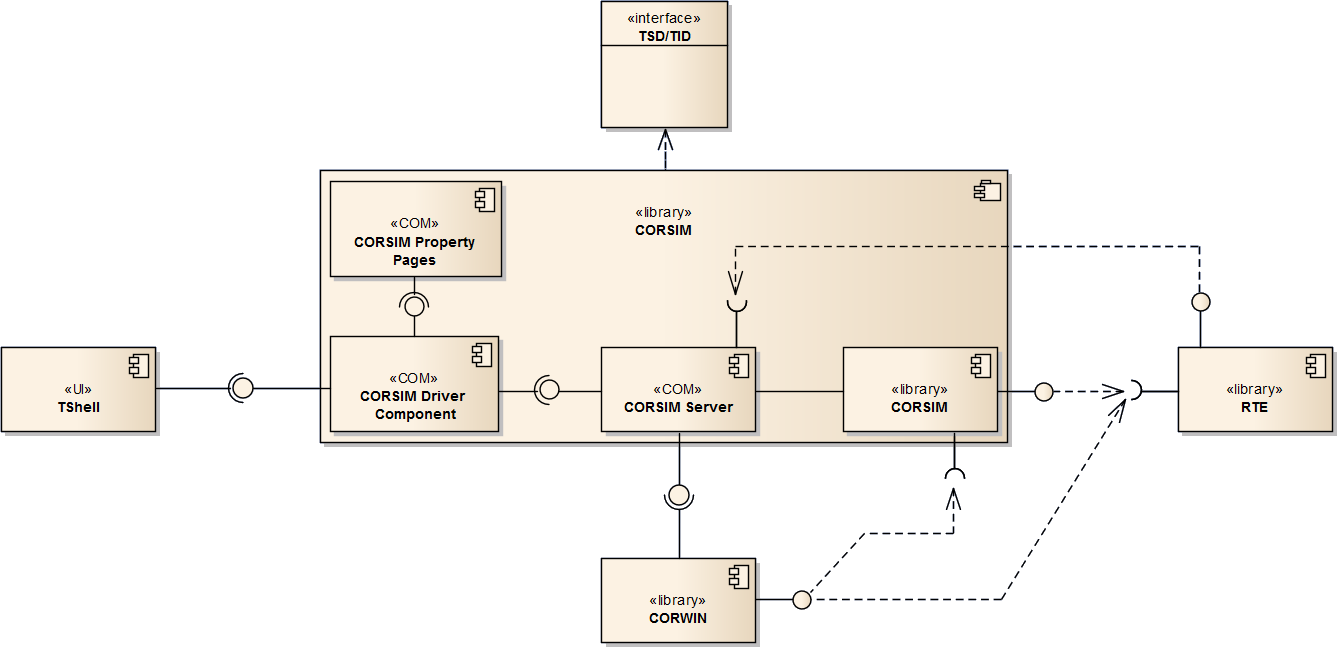
\includegraphics[width=1\columnwidth]{tsis-corsim-components}
\caption[Diagramma dei componenti di \acs{CORSIM}]{Porzione del diagramma dei componenti di \acs{TSIS}: mostra l'architettura modulare e il funzionamento di \acs{CORSIM} all'interno di \acs{TSIS}.}
\label{fig:tsis-corsim-arch}
\end{sidewaysfigure}

Anche se la~\vref{fig:tsis-corsim-arch} mostra per completezza l'intera architettura di \acs{CORSIM}, si procede con la descrizione delle interfacce di \acs{CORSIM} preposte alla comunicazione con \acs{RTE} sviluppate dall'utente, identificate dalle frecce tratteggiate.

\subsubsection{CORWIN}

\subsubsection{CORSIM API}

Required Tools
This section describes the tools needed for successful compilation of a CORSIM run-time extension. Building a
CORSIM RTE requires a suitable compiler such as Microsoft Visual C++ or FORTRAN and the TSIS package,
which includes all of the components shown in the previous figure (except for the RTE).

\section{Estensione}
% TODO: introduzione, problema che deve risolvere
% massima granularità dell'output dei sensori: 1 secondo . non va bene, quindi estensione Sensors ..

\subsection{Analisi}
% TODO: analisi del problema e del software che si è realizzato

\subsection{Sensors DLL}
% TODO: presentazione della DLL, progetto del software?

\section{Applicativi di supporto}
% TODO: discussione sulle operazioni utili alla creazione di dataset: insieme di file, ognuno dei quali è un insieme di traiettorie multivariate
